%%%%%%%%%%%%%%%%%%%%%%% file typeinst.tex %%%%%%%%%%%%%%%%%%%%%%%%%
%
% This is the LaTeX source for the instructions to authors using
% the LaTeX document class 'llncs.cls' for contributions to
% the Lecture Notes in Computer Sciences series.
% http://www.springer.com/lncs       Springer Heidelberg 2006/05/04
%
% It may be used as a template for your own input - copy it
% to a new file with a new name and use it as the basis
% for your article.
%
% NB: the document class 'llncs' has its own and detailed documentation, see
% ftp://ftp.springer.de/data/pubftp/pub/tex/latex/llncs/latex2e/llncsdoc.pdf
%
%%%%%%%%%%%%%%%%%%%%%%%%%%%%%%%%%%%%%%%%%%%%%%%%%%%%%%%%%%%%%%%%%%%


\documentclass[runningheads,a4paper]{llncs}

\usepackage{amssymb}
\setcounter{tocdepth}{3}
\usepackage{graphicx}
%%%%%%%%%%%%%%% New package
\usepackage{amsmath}
\usepackage{caption}
\usepackage{subfig}
\usepackage{csvsimple}
\usepackage{multirow}
\usepackage{array}
\usepackage{booktabs}
\usepackage{listings}
%%%%%%%%%%%%%%%
\usepackage{url}
% \urldef{\mailsa}\path|{soltanin, locheng, ingrid.haas, frank.holzwarth,|
% \urldef{\mailsb}\path|anna.kramer, leonie.kunz, christine.reiss, nicole.sator,|
% \urldef{\mailsc}\path|erika.siebert-cole, peter.strasser, lncs}@springer.com|
% \newcommand{\keywords}[1]{\par\addvspace\baselineskip
% \noindent\keywordname\enspace\ignorespaces#1}
\usepackage{indentfirst}
\setlength{\parindent}{2em}
\begin{document}

%\mainmatter  % start of an individual contribution

% first the title is needed
\title{Analysis of LIDAR Point Cloud Data Using Poisson Surface Reconstruction}

% a short form should be given in case it is too long for the running head
%\titlerunning{Lecture Notes in Computer Science: Authors' Instructions}

% the name(s) of the author(s) follow(s) next
%
% NB: Chinese authors should write their first names(s) in front of
% their surnames. This ensures that the names appear correctly in
% the running heads and the author index.
%
\author{Ruoyang Song, Jianfei Ma, Tao Han, Arturo Sanchez-Azofeifa, Anup Basu}
%\thanks{Please note that the LNCS Editorial assumes that all authors have used
%the western naming convention, with given names preceding surnames. This determines
%the structure of the names in the running heads and the author index.}%

%%
%\authorrunning{Lecture Notes in Computer Science: Authors' Instructions}
% (feature abused for this document to repeat the title also on left hand pages)

% the affiliations are given next; don't give your e-mail address
% unless you accept that it will be published
\institute{Dept. of Computing Science, University of Alberta, Canada}

%
% NB: a more complex sample for affiliations and the mapping to the
% corresponding authors can be found in the file "llncs.dem"
% (search for the string "\mainmatter" where a contribution starts).
% "llncs.dem" accompanies the document class "llncs.cls".
%

% \toctitle{Lecture Notes in Computer Science}
% \tocauthor{Authors' Instructions}
\maketitle


\begin{abstract}
Tree volumes play a significant role in analyzing the bioinformation of a forest. It provides biologists ground truth to analyze the change in biodiversity according to the number of species and their distribution. Light Detection and Ranging (LiDAR) scanning can be used to scan large multi-hectare areas of forests with thousands of trees. During the past decades, computer scientists have been working on calculating the volume of tree buttresses of the point cloud data gathered from LiDAR system. In this paper, we investigate into several point cloud segmentation algorithms for dividing the irregular shaped buttress into regular shaped object for calculation, and we promote a new method for analyzing the volume using Poisson Surface Reconstruction algorithm.  Our proposed method has four main steps: 1) Removing outliers using a Statistical Outlier Removal filter, 2) Computing normals of the point clouds, 3) Applying the Poisson Surface Reconstruction algorithm to the point cloud, 4) Calculating the mesh volume. We examinated Euclidean Cluster Extraction algorithm and Cylinder segmentation algorithm for irregular shaped buttresses.
\end{abstract}


\section{Introduction}
For decades, scientists have been dedicated for calculating the accurate volume of tree buttresses from point cloud data. For the tree branches, there are already some good segmentation algorithms such as QSM used to calculate the volumes. However, the volume calculation for the buttresses part is still a difficult problem due to the complexity a buttress can have. The volume of tree buttress can contribute significantly in multiple fields of studies. For example, biologists can analyze the basic bioinformation of this forest and species may live inside it. In addition to that, the detailed tree species data can be used for biologists to analyze the changes in biodiversity according to the number of species and their distribution. Scientists with different background have been approaching this problem using all kinds of technologies.
First of all, a vast majority of research effort in tree species recognition has been devoted to retrieve the tree texture and how to match to the acknowledged database. In 2004, Norbert Haala and his fellow coauthors derived geometric quantities like position and diameter of trees from the IMAGER 5003 LIDAR system, and texture parameters from the high resolution panoramic imagery shoot by a EYSCAN camera \cite{1}. From the result, we can see that since the texture differs between stems, using only texture to identify tree species is a novel approach but has a limited correct rate. And in 2013, Othmani improved this methodology by using the 3D geometric texture of the bark, rather than 2D texture from imagery. Othmani computed the texture features using a combination of the Complex Wavelet Transforms (CWT) and the Contourlet Transform (CT), and classification was done using the Random Forest (RF) classifier. 
After testing using a dataset composed of 230 samples, even the worst average overall accuracy has been increased to 80.62\% (with a standard deviation of 5.82\%) \cite{2}.
Secondly, hyperspectral data is also widely used in analyzing tree species. In 2010, Puttonen collected a database contains the shape parameters of three boreal tree species which is merged from two dataset: One is actively scanned hyperspectral point cloud, and the second one is collected with a spatially accurate LIDAR \cite{3}. The result shows a huge increase in correct rate compared to previous methodology: With a combination of 2 features from each dataset, the average classification accuracy was over 85\% for all species. And in 2013, Vauhkonen improved the tree species classification methodology by analyzing the hyperspectral reflectance that had penetrated through the foliage \cite{4}. In this study, he focused on the species-specific differences as recorded by an active hyperspectral LiDAR in a laboratory measurement of pine and spruce trees. He divided the reflectance values into several categories based on Normalized Difference Vegetation Index (NDVI) and reflectance losses. And by analyzing the pulse penetration and reflectance, he got a 78\% to 97\% of correct rate on 18 spruce and pine trees.
Lastly, in the latest study done by Åkerblom in 2017, not like any other study done before, he did not start from using the 3D point cloud data directly, trees are first reconstructed as quantitative structure models (QSM) \cite{5}. For each tree, the QSM reconstruction process creates another partition of the tree point cloud into small patches, and then segments them into the stem and branches. Then he computed a scalar value for each QSM model, and match them with a table of tree features as shown in Figure 1. In this way, based on applying this methodology to 1200 trees in different species, it shows a quite convincing result of an average classification accuracy above 93\%.
However, all these methodologies mentioned share one hypothesis: the assumption that all the trees’ bottom part look like cylinder. However, there are still many other trees that have buttress root lives on earth. Applying above methodologies to trees that have buttress root may lead to a biased result. As a result, we will focus on how to improve the classification accuracy to trees with buttress root.
divide an irregular shaped buttress into several cylinder objects or Euclidean Cluster. We assumed that it must be approachable for calculating the accurate volume of these segmented regular shaped objects using convex hull algorithm. However, the result we got has a significant deviation with reality and this biased result does not support us in the next step of calculating the accurate value of the buttress. As a result, we moved to a new approach using Poisson Surface Reconstruction. Our goal is to calculate the result as accurate as possible. The general steps of the proposed method include removing outliers using a Statistical Outlier Removal filter, computing normal of the point clouds, apply the Poisson Surface Reconstruction algorithm to the point cloud, and calculate the mesh volume.
The remaining sections of this paper are structured as follows: Section 2 covers materials, which provides details on the dataset. Section 3 lists some previous work related to our topic. Section 4 concludes our abortive methods, which may still be an inspiration for the final implementation. Section 5 is the preprocessing and the proposed method for calculating the volume of an irregular shaped buttress using Poisson Surface Reconstruction. We also give an example experiment. The experimental results and discussion are also covered in Section 5. Finally, Section 6 presents the conclusion.




\section{Data Set}
The point cloud data used in the preparation of this article was collected from scanning two tree samples using LiDar camera. We will give two sample trees for experiments. As shown in the Fig.\ref{fig:easy-tree-sample}, the first tree sample has a straight brunch which allow us to reconstruct it into a cylinder easily. On the controversy, the another tree sample has a complicated irregular shaped buttress structure as shown as Fig.\ref{fig:complex-tree-sample}.

\begin{figure}
\begin{minipage}{.5\textwidth}
  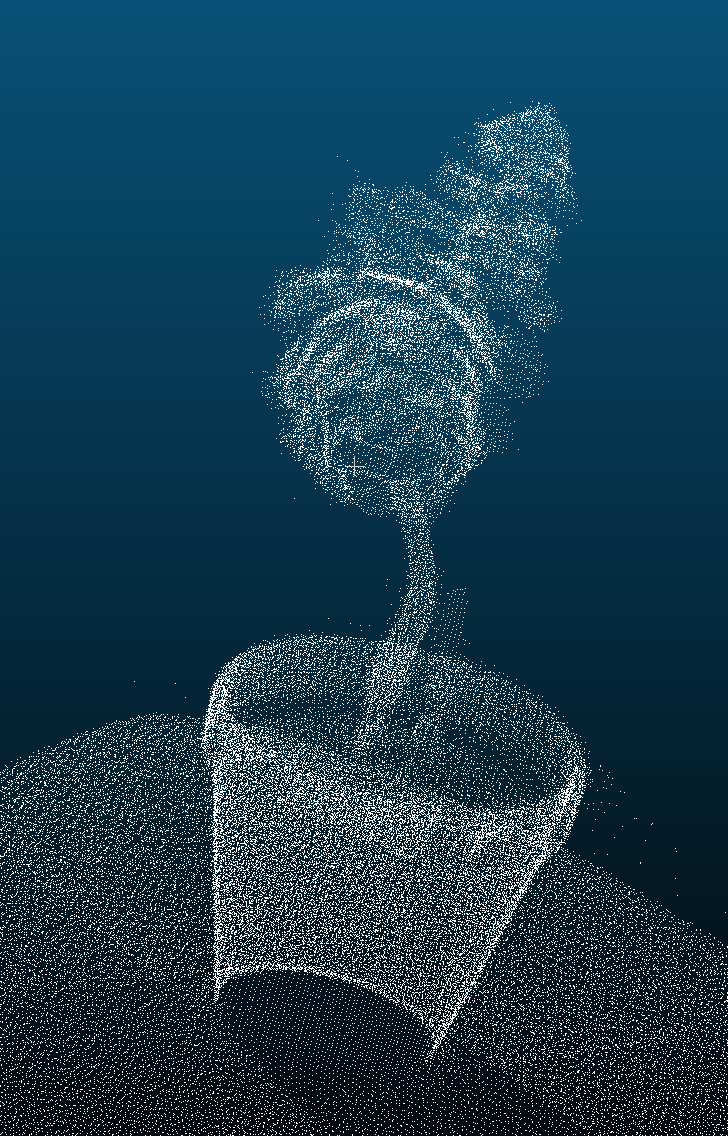
\includegraphics[width=.6\linewidth]{easy-tree-sample.png}
  \captionof{figure}{Regular shaped brunch.}
  \label{fig:easy-tree-sample}
\end{minipage}
\begin{minipage}{.5\textwidth}
  \centering
  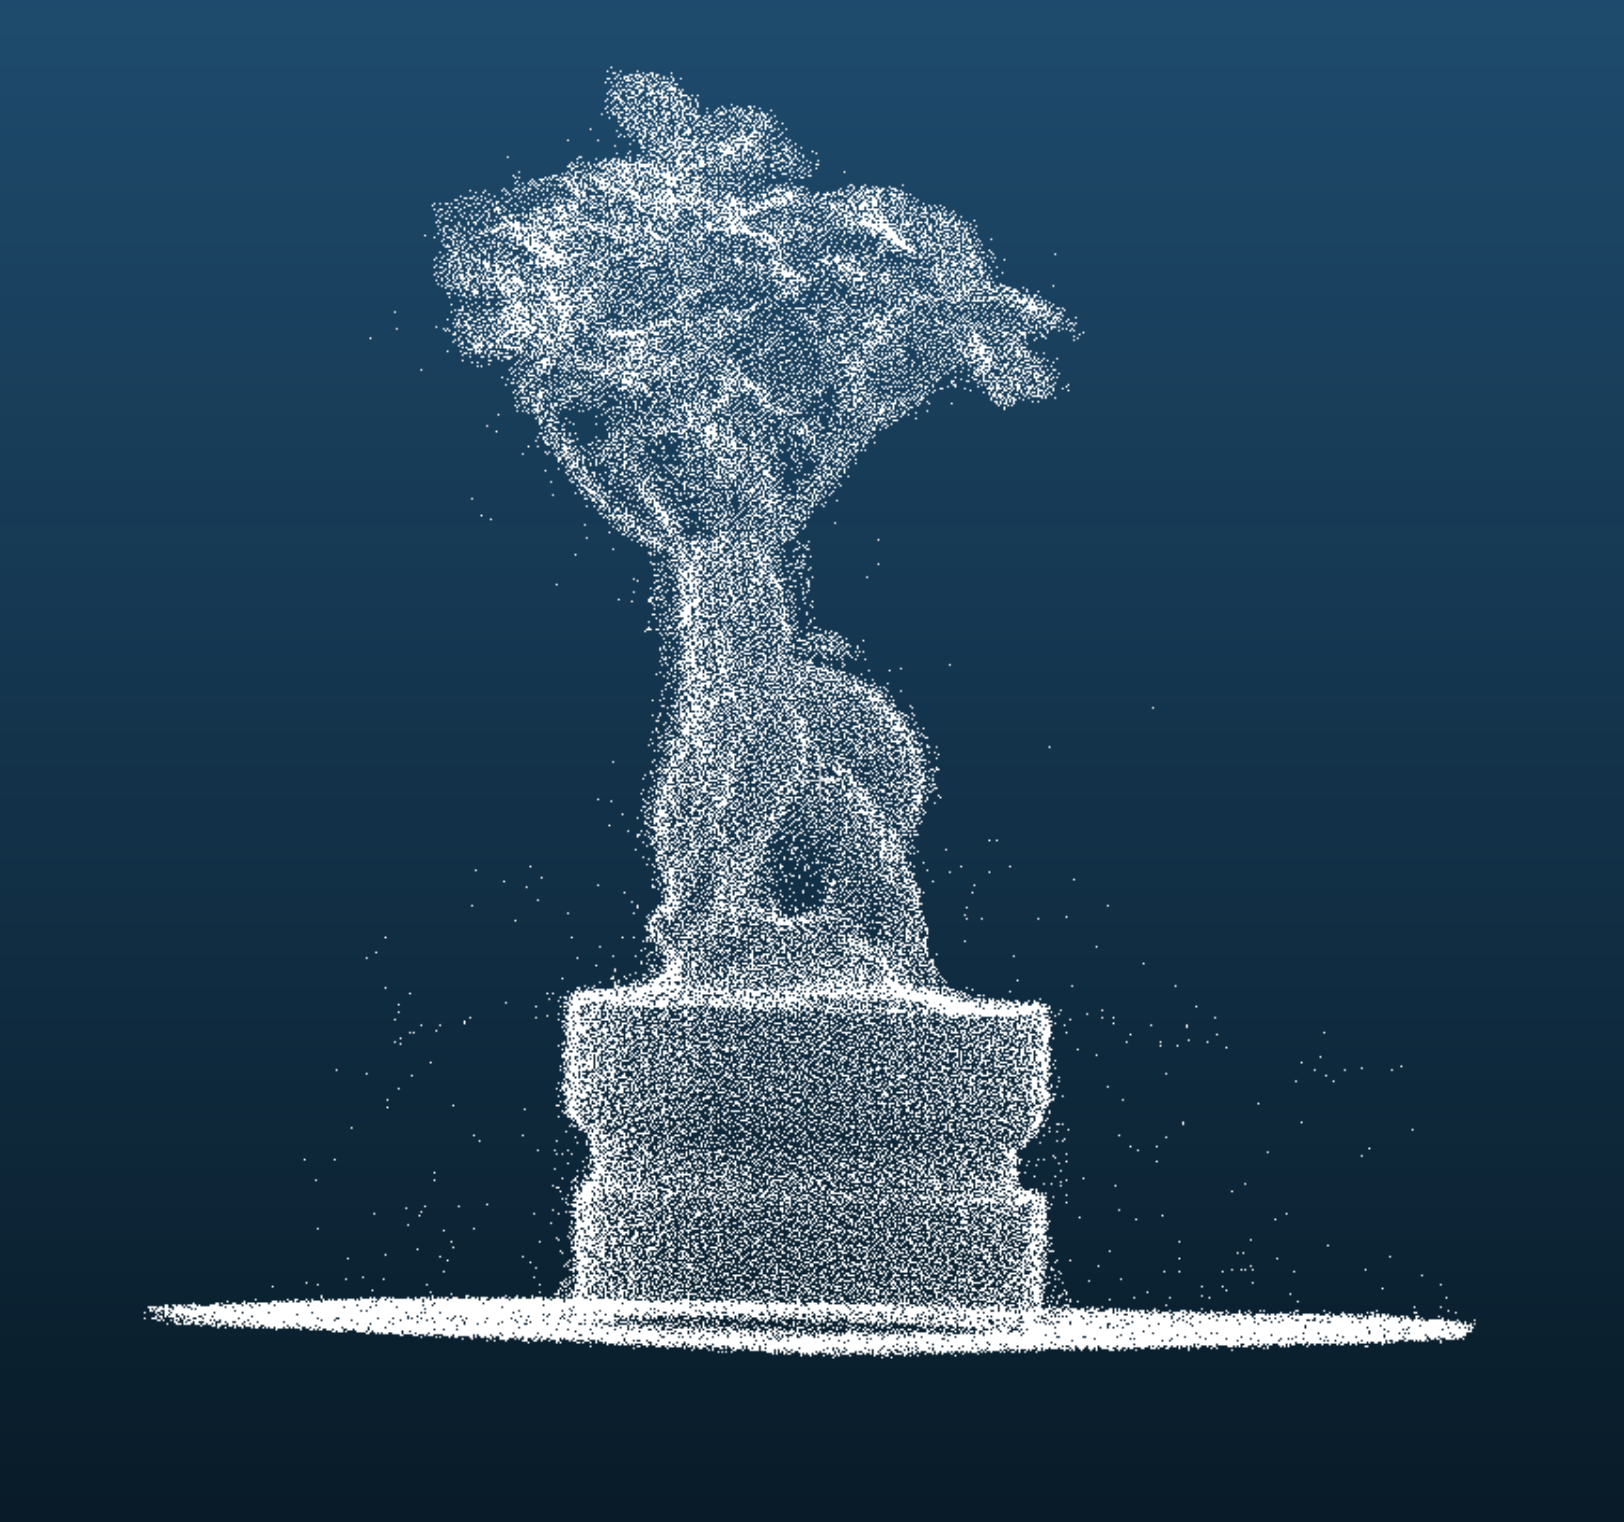
\includegraphics[width=1\linewidth]{complex-tree-sample.png}
  \captionof{figure}{Irregular shaped buttress.}
  \label{fig:complex-tree-sample}
\end{minipage}
\end{figure}

\section{Related Work}
\subsection{The existing structure recognizing method for point clouds}
\subsubsection{Introduction}
G. Vosselman, B.G.H. Gorte, G. Sithole and T. Rabbani(2004) introduced different techniques for recognising structure in point cloud in Recognising Structure in Laser Scanner Point Clouds \cite{6}. Using these methods, we can extract planar surfaces and specific shapes in point clouds. As they mentioned, the objects under study are polyhedral in most case. For our project, some buttresses can be studied as polyhedral once we segment them into small prisms or cylinders. They introduced a direct extraction method for parameterised shapes including planes, cylinders and spheres. We may be interested in the cylinder part for our project. A cylinder usually be described by five parameters. The number of bins of cylinders caused a needless time and memory consuming and unreliable. Hence, they reduce the dimension of the parameter space into two parts: the detection of the cylinder axis direction and detection of a circle in plane. By extracting the circle parts with high counters along the larger part of it, hypothesis for cylinder axis directions are confirmed. As they mentioned, the application has been applied on the tree structure recognising, “as a result, to each point a label is assigned that is unique for each branch, whereas points are removed that do not belong to the stem or a significant branch.”  Their applications are shown in Fig.\ref{fig:simple tree recognition}.
\begin{figure}
\begin{minipage}{.5\textwidth}
  \centering
  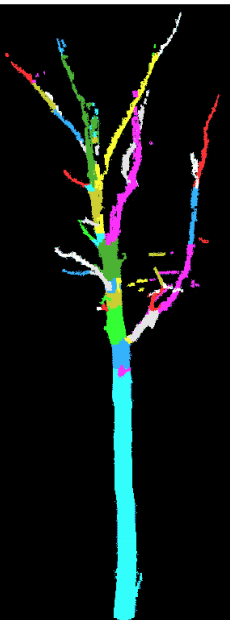
\includegraphics[width=.3\linewidth]{The_existing_segmentation.png}
  \captionof{figure}{Simple tree recognition.}
  \label{fig:simple tree recognition}
\end{minipage}
\begin{minipage}{.5\textwidth}
  \centering
  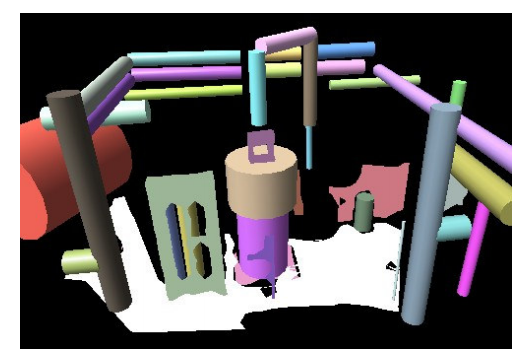
\includegraphics[width=1\linewidth]{Cylinders_and_planes.png}
  \captionof{figure}{Segmentation in an industrial scene.}
  \label{fig:segmentation}
\end{minipage}
\end{figure}
\subsubsection{Limitation}
This method performs good in recognizing tree branches and simple tree buttress roots. However, for most tropical tree, the shapes of their buttress roots are quite random and cannot be simply generalized as several surfaces, spheres or cylinders. For a complex tree buttress shown below, this method may lead to a wrong segmentation in the point cloud.
\\
\begin{minipage}{1\linewidth}
  \centering
  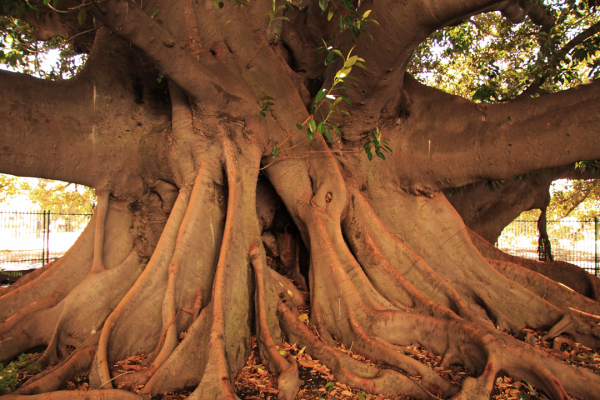
\includegraphics[scale=1]{complex_buttress.jpg}
  \captionof{figure}{Complex tree buttress roots.}
  \label{fig:Complex tree buttress}
\end{minipage}

\subsection{Existing algorithms for determining minimum Convex Polygon (Convex Hull)} 
\subsubsection{Introduction}
For volume calculating, the Convex Hull algorithm maybe helpful. Since year 1970,  the first article about determining minimum convex polygon has been published \cite{7}, mathematicians and computer scientist started to realize that computing the convex hull means that a non-ambiguous and efficient representation of the required convex shape can be constructed. With this property, algorithms for constructing convex hulls of various objects have a broad range of applications in mathematics and computer science. For example, in the Simplex Algorithm, the optimal point was found by iterating over the vertices of the convex hull constructed from the linear constraints. And in recent years, scientist has published several algorithms for this topic, and most them have a average time complexity of O(n log n) where n stands for the the number of inputs points.

\begin{minipage}{\linewidth}
  \centering
  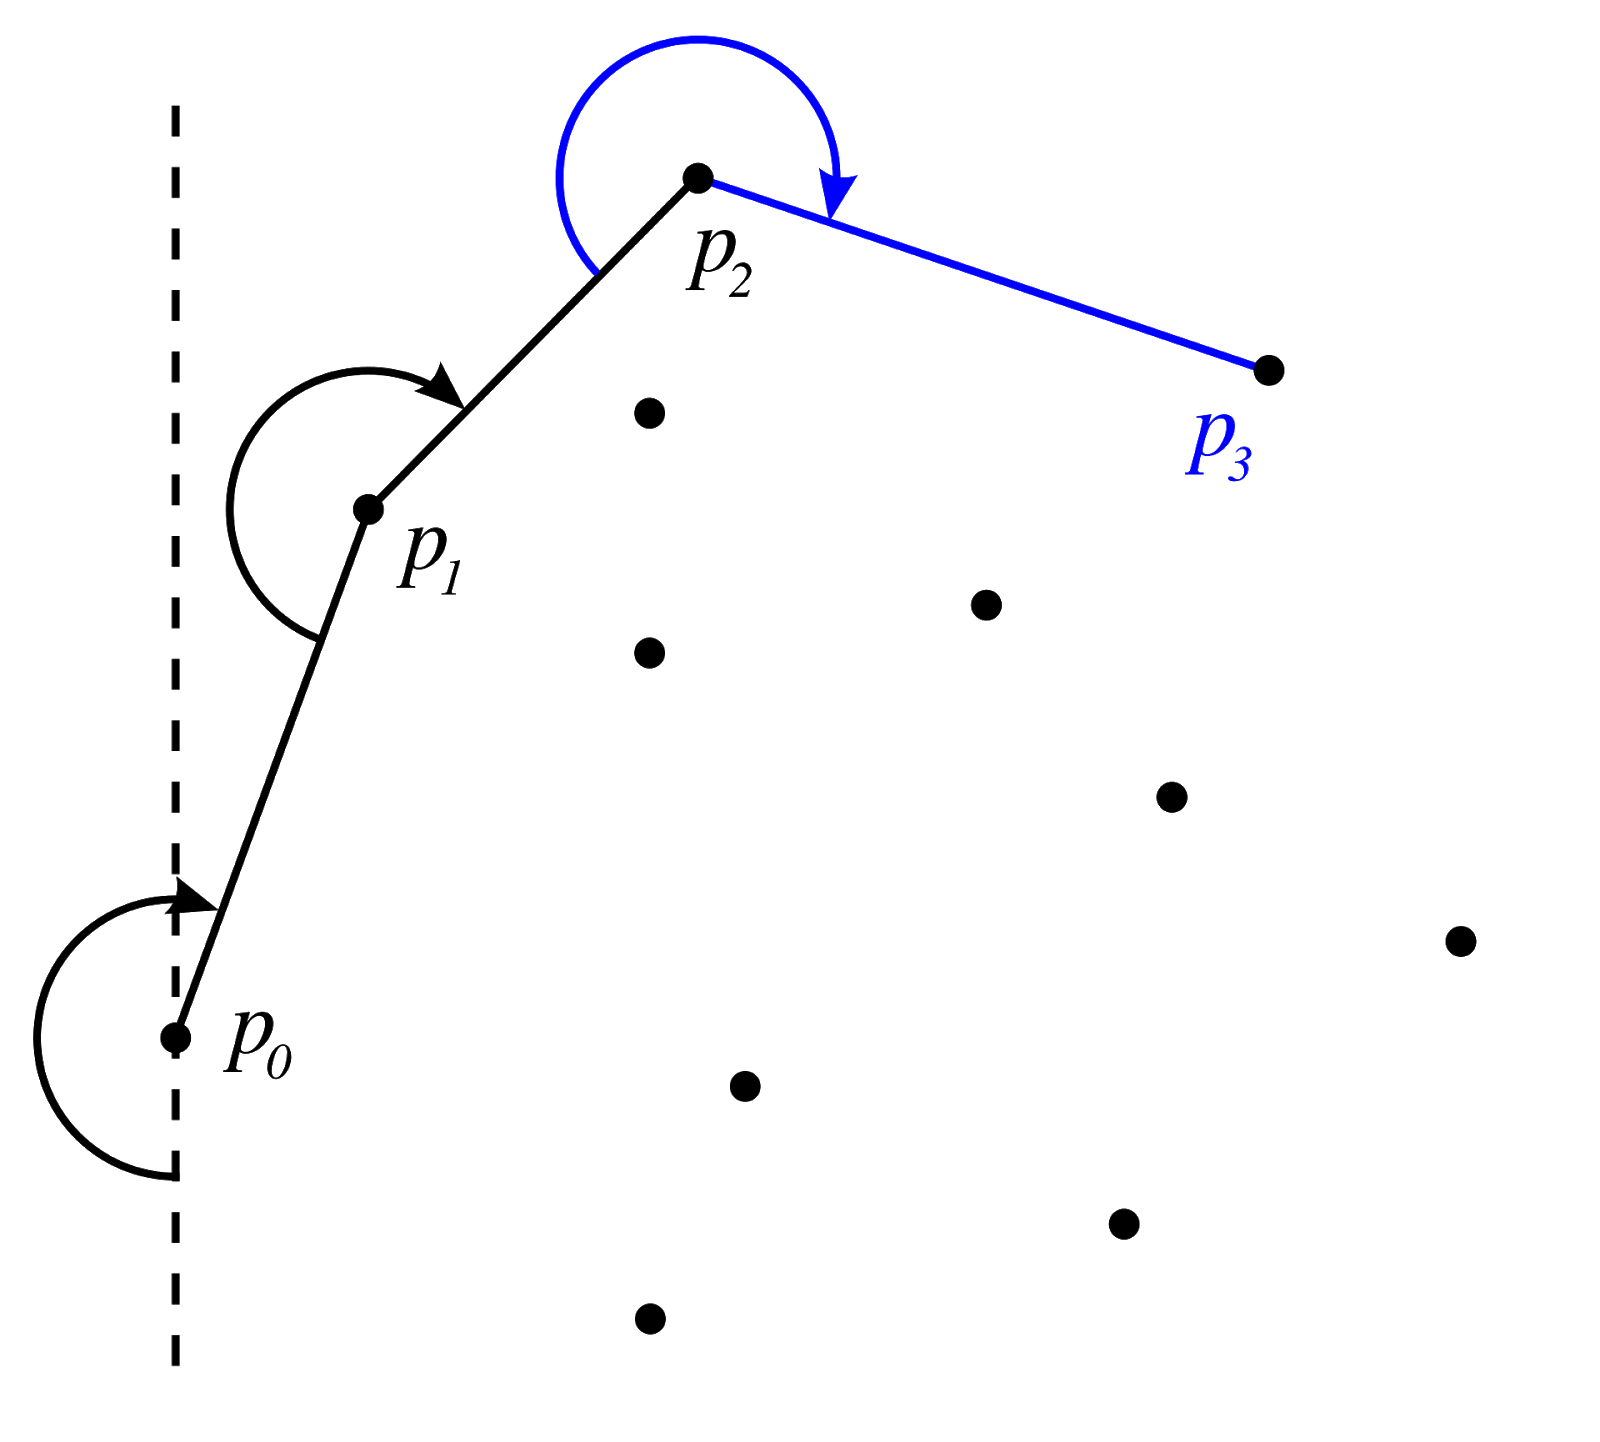
\includegraphics[scale=.1]{ConvexHull1.png}
  \captionof{figure}{Example of Gift Wrapping Algorithm.}
  \label{fig:ConvexHull1}
\end{minipage}

As the first algorithm published for determining minimum convex hull, the Gift Wrapping \cite{7} is one of the simplest algorithm,  also as known as Jarvis march.  Donald R. Chand published this algorithm in 1970, and as shown in Figure 2, this algorithm starts from the left-most point and try to find the next point which have the largest polar angle. This algorithm has a O(nh) time complexity where n is the number of points and h is the number of points on the convex hull. Although it’s not the most time efficient in the worst case, if we have an expected small number of points, this algorithm can have better performance and faster computation time compared to other algorithms.
All the Convex Hull algorithms before 1996 can only be applied to 2D points and detect a planar convex hull. Since our research object is the 3D position data of a tree, we need to used the Chan’s algorithm published \cite{8}. This algorithm is not restricted to 2D anymore, it naturally extended to 3D space and can be used for find the convex hull of a 3D point cloud. This algorithm starts by arbitrarily partitioning the set of points into several subset, and then use Graham Scan to compute the convex hull for each subset. The average time complexity of this algorithm is  O(n log h), where n stands for the number of points and h stands for the number of vertices of the final convex hull. Since this algorithm meets all the requirement of this research project, we decide to use this algorithm to find the convex hull of our tree point cloud data.

\subsubsection{Limitation}
The Convex Hull algorithm will connect all the points in our point cloud. The result that applying the Convex Hull on our sample buttress roots is shown in Fig.\ref{fig:ConvexHull3}. Obviously, there will be a huge bias if we apply Convex Hull directly to calculate the volume. Hence, we need a good clustering algorithm that performs good on complex tree buttresses that we can apply the algorithm on each cluster. However, it is difficult to find a clustering algorithm that works good on tree buttress roots.
\begin{figure}
\begin{minipage}{.5\textwidth}
  \centering
  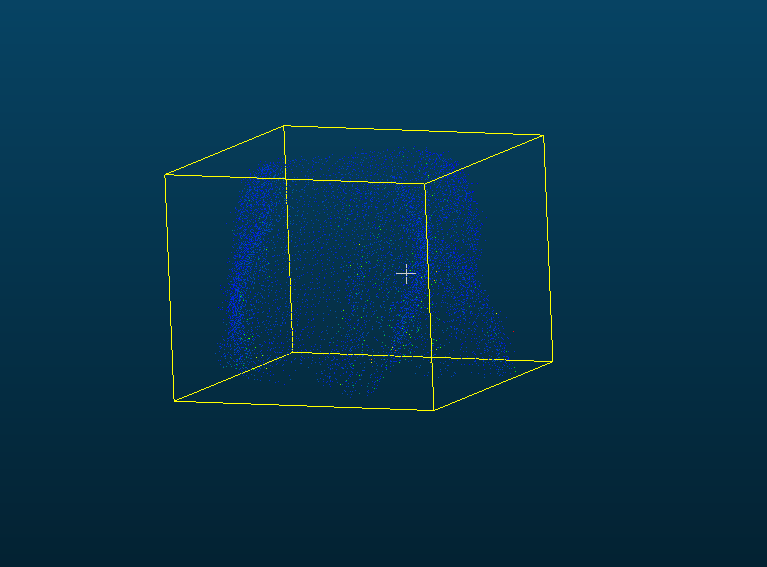
\includegraphics[width=1\linewidth]{ikea_buttress_SOR.PNG}
  \captionof{figure}{A sample tree buttress.}
  \label{fig:A sample tree buttress}
\end{minipage}
\begin{minipage}{.5\textwidth}
  \centering
  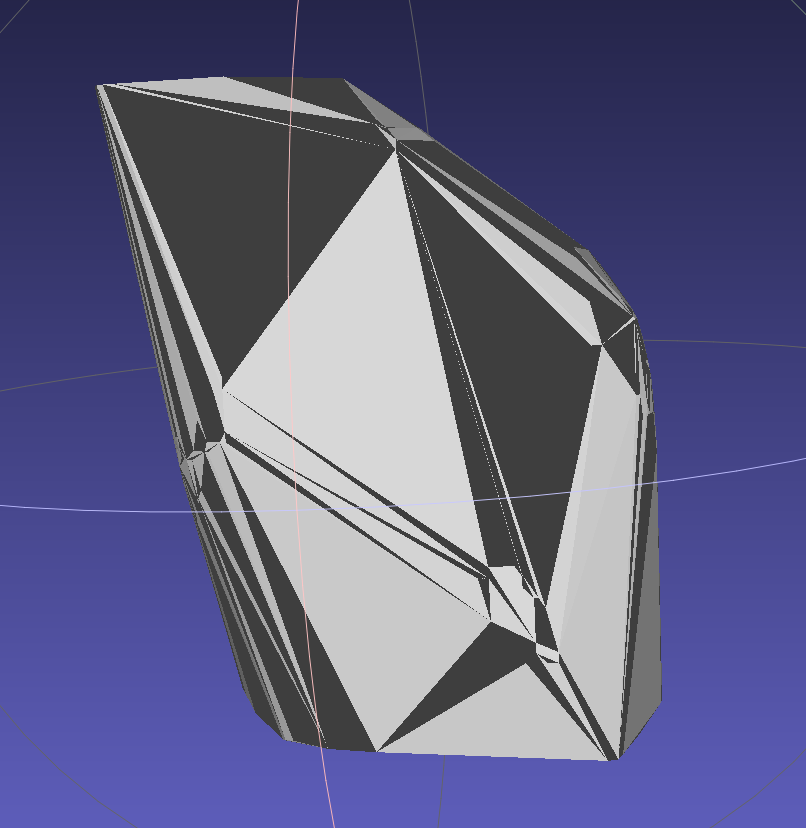
\includegraphics[width=.7\linewidth]{Convex.PNG}
  \captionof{figure}{Sample buttress with Convex Hull}
  \label{fig:ConvexHull3}
\end{minipage}
\end{figure}


\section{Abortive Experiments}
Since we focused on analyzing the point cloud of irregular shaped data, our first approach was to segment the irregular shaped part into smaller objects with regular shapes. 
\subsection{Euclidean Cluster Extraction algorithm}
Euclidean clustering essentially groups points that are close together. We set a "closeness" threshold, such that points within this threshold are considered to be part of the same cluster. We also set a minimum and a maximum number of points that a cluster can contain. This helps us to filter out noise (isolated single points) or parts of the surface that were not segmented out \cite{9}. The outline of this algorithm is:
\begin{enumerate}
\item Create a Kd-tree representation for the input point cloud dataset P.
\item Set up an empty list of clusters C , and a queue of the points that need to be checked Q.
\item For every point p in P , perform the following steps:
\begin{enumerate}
\item Add p to the current queue Q.
\item	For every point p in Q do:
\begin{enumerate}
\item Search for the set of point n neighbors of p in a sphere with radius r.
\item For every neighbour n , check if the point has already been processed, and if not add it to Q.
\end{enumerate}
\item When the list of all points in Q has been processed, add Q to the list of clusters C, and reset Q to an empty list
\end{enumerate}
\item The algorithm terminates when all points p have been processed and are now part of the list of point clusters C
\end{enumerate}

From the Fig.\ref{fig:Euclidean-cluster}, we can see that the tree sample was segmented into several Euclidean Cluster. However, we have to manually set up parameters for threshold and maximum number of points, and these two parameters vary from one tree to another, which indicates that this approach can not be generalized to all buttress without manual operation. 

\begin{figure}
\centering
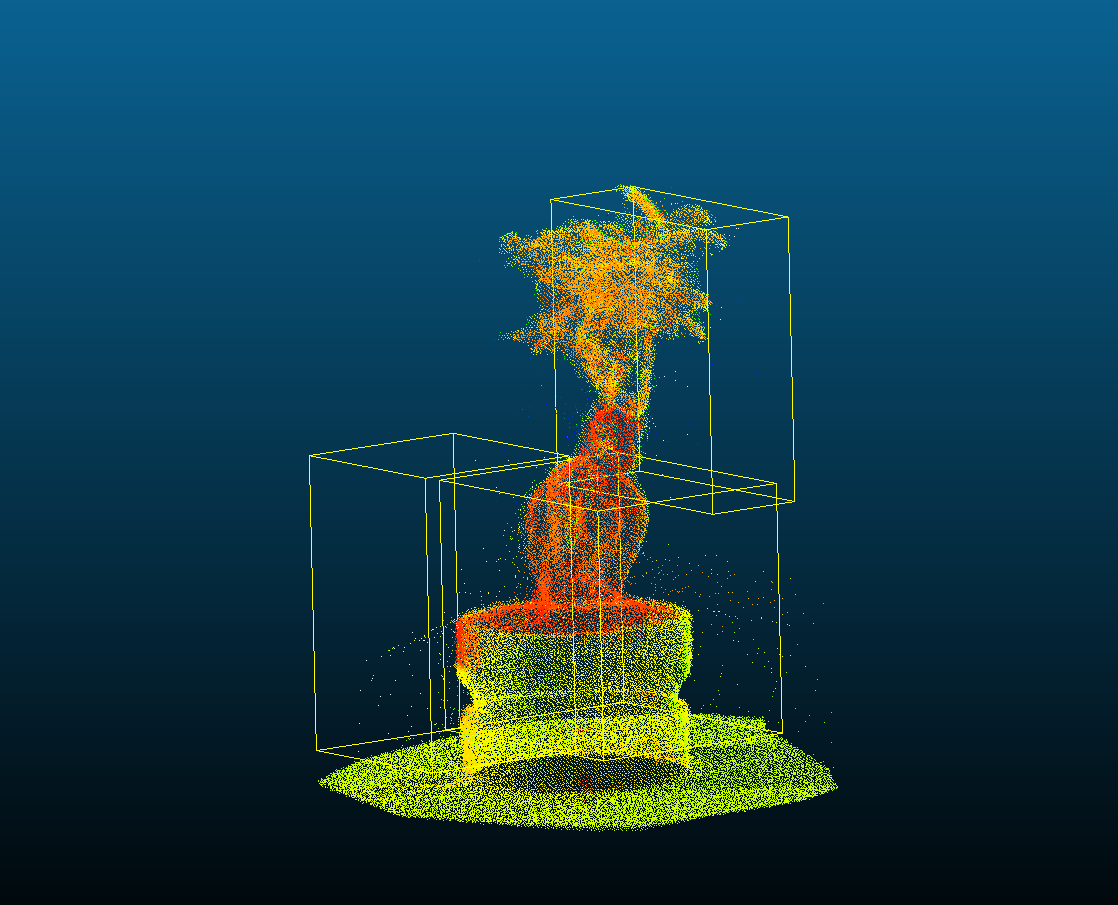
\includegraphics[scale=0.6]{Euclidean-cluster-extraction-result.png}
\caption{Result for applying the Euclidean Cluster Extraction algorithm to the complex tree sample.}
\label{fig:Euclidean-cluster}
\end{figure}

\subsection{Cylinder segmentation algorithm}
In 2014, Trung-Thien Tran published his Sample Consensus Segmentation algorithm for extraction of cylinders and estimation of their parameters from point clouds \cite{10}. Since this algorithm is widely used in multiple fields of point cloud analyzing industry, we can use this algorithm from PCL library.


\begin{figure}
\centering
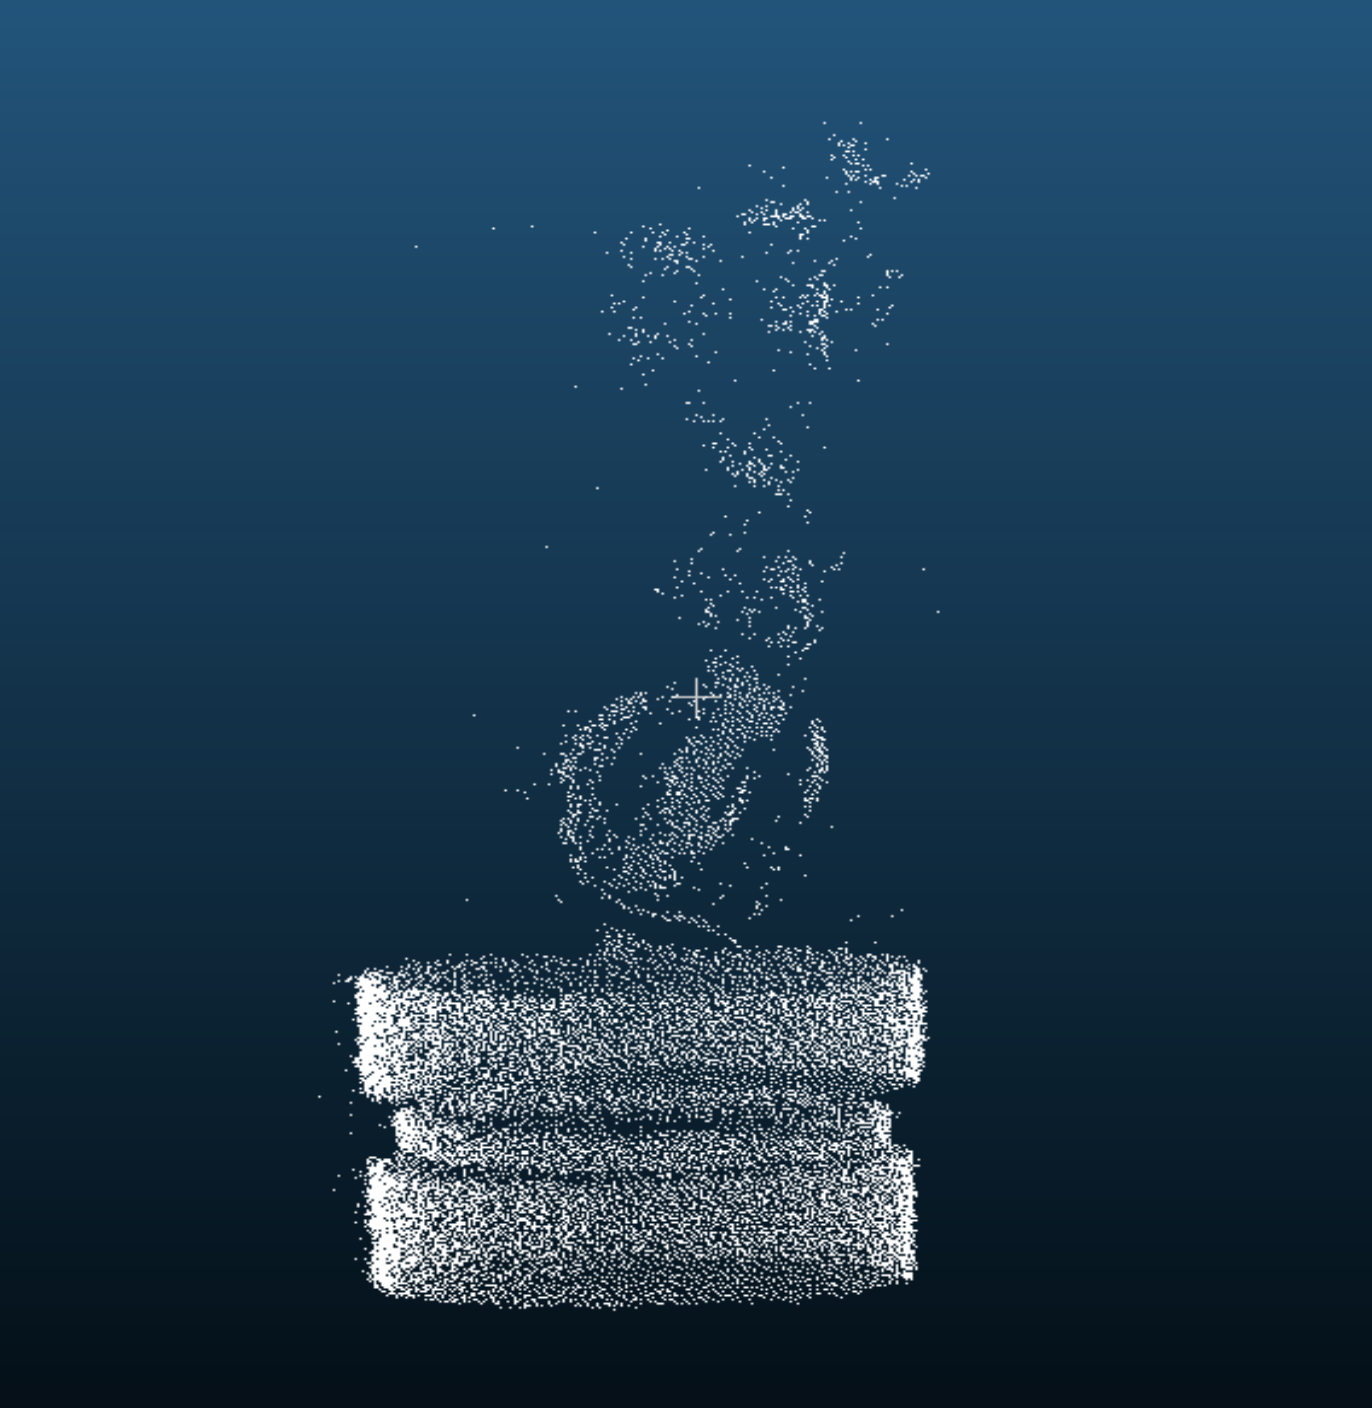
\includegraphics[scale=0.3]{cylinder-extraction-result.png}
\caption{Result from Sample Consensus Segmentation algorithm}
\label{fig:cylinder-extraction-result}
\end{figure}

However, from Fig. \ref{fig:cylinder-extraction-result},  we can see this algorithm does not perform very well. The reason behind this is that the buttress part of the point cloud data we collected was intertwined into together, and it does not contains a relatively big empty space between each buttress. This Sample Consensus Segmentation algorithm should have better performance for a tree like Fig. \ref{fig:widespread-buttress}.

\begin{figure}
\centering
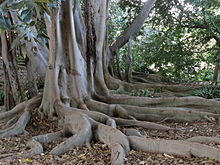
\includegraphics[scale=.5]{Buttress_roots.JPG}
\caption{Tree with widespread buttress }
\label{fig:widespread-buttress}
\end{figure}


\section{Proposed Method}
There are three general steps included in out proposed methods: 

The overview of our proposed method is presented in Fig.\ref{fig:framework}  which has $3$ general steps including: (1) Preprossing (2) Computing normals of the point clouds (3) Applying the Poisson Surface Reconstruction algorithm to the point cloud (4) Segmenting out the buttress part and close holes (5). Calculating the mesh volume. Next, each step is explained in detail. 

\begin{figure}
\centering
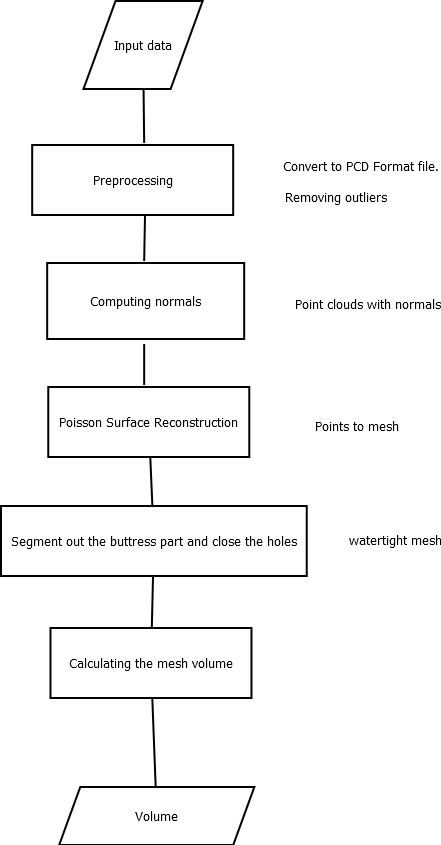
\includegraphics[scale=.35]{framework.PNG}
\caption{Framework}
\label{fig:framework}
\end{figure}

\subsection{Preprossessing}
Preprocessing is a fundamental step of calculating the accurate volume of a tree point cloud. In this paper, for reconstructing a meticulous mesh using the point cloud, two prepossessing steps are needed. 
\subsubsection{Convert To PCD Format}
Since the point cloud data we collected was initially stored in TXT format, we need to convert our data into PCD format for the following advantages over other file format \cite{11}:
\begin{enumerate}
\item the ability to store and process organized point cloud datasets – this is of extreme importance for real time applications, and research areas such as augmented reality, robotics, etc;
\item binary mmap/munmap data types are the fastest possible way of loading and saving data to disk.
\item storing different data types (all primitives supported: char, short, int, float, double) allows the point cloud data to be flexible and efficient with respect to storage and processing. Invalid point dimensions are usually stored as NAN types.
\item n-D histograms for feature descriptors – very important for 3D perception/computer vision applications
\end{enumerate}


\subsubsection{Removing outliers using a Statistical Outlier Removal filter}
The point cloud data gathered from Laser scans has a varying point densities. Also, there are some measurement errors which may cause visible outliers. The varying densities and outliers will lead to bias, and make our further steps such as normal calculation complicated. We are going to apply a Statistical Outlier Removal filter on our point clouds.

Our sparse outlier removal is based on the computation of the distribution of point to neighbors distances in the input dataset. For each point, we compute the mean distance from it to all its neighbors. By assuming that the resulted distribution is Gaussian with a mean and a standard deviation, all points whose mean distances are outside an interval defined by the global distances mean and standard deviation can be considered as outliers and trimmed from the dataset\cite{12}.

The following picture Fig. \ref{fig:SOR} shows the effects of applying SOR filter on a point cloud. The graphic shows the mean k-nearest neighbor distances in a point neighborhood before and after filtering\cite{12}.

\begin{figure}
\centering
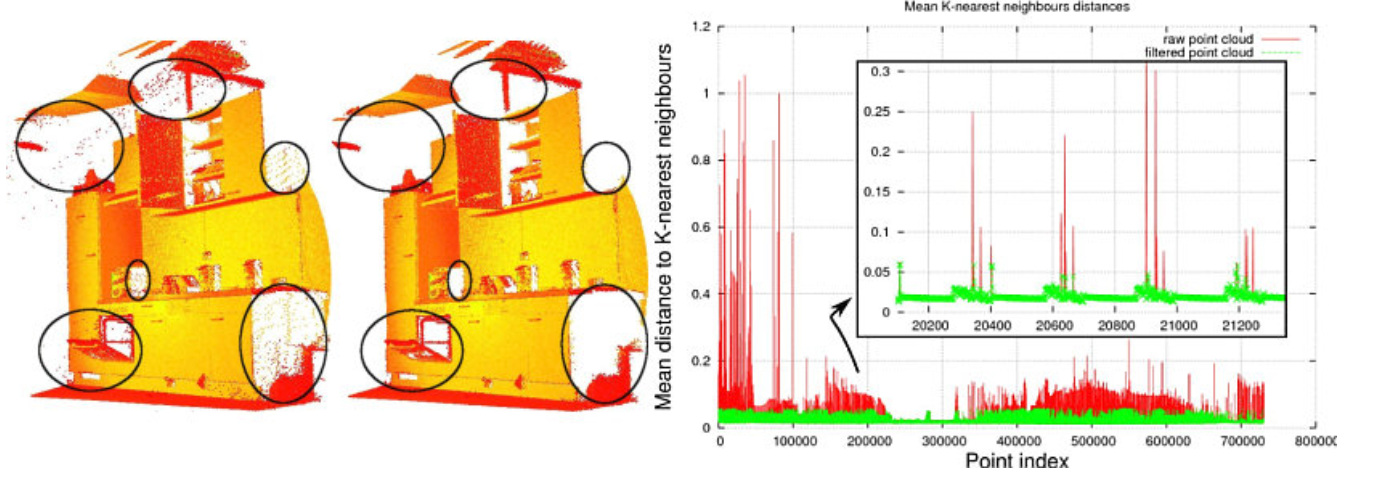
\includegraphics[scale=.7]{SOR.PNG}
\caption{The SOR result from PCL documentation}
\label{fig:SOR}
\end{figure}

After we convert our point cloud into PCD format, we remove the noise in the point cloud for generating a meticulous mesh in the next step. We will perform the Statistical Outlier Removal filter from PCL library in this step \cite{13}:

We can see the comparison before and after removing the outliers from Fig.  \ref{fig:fiiter-comparison}. All the outliers which are floating outside of the main object is removed and the result is good start point for generating the mesh.

\begin{figure}
\begin{minipage}{.5\textwidth}
  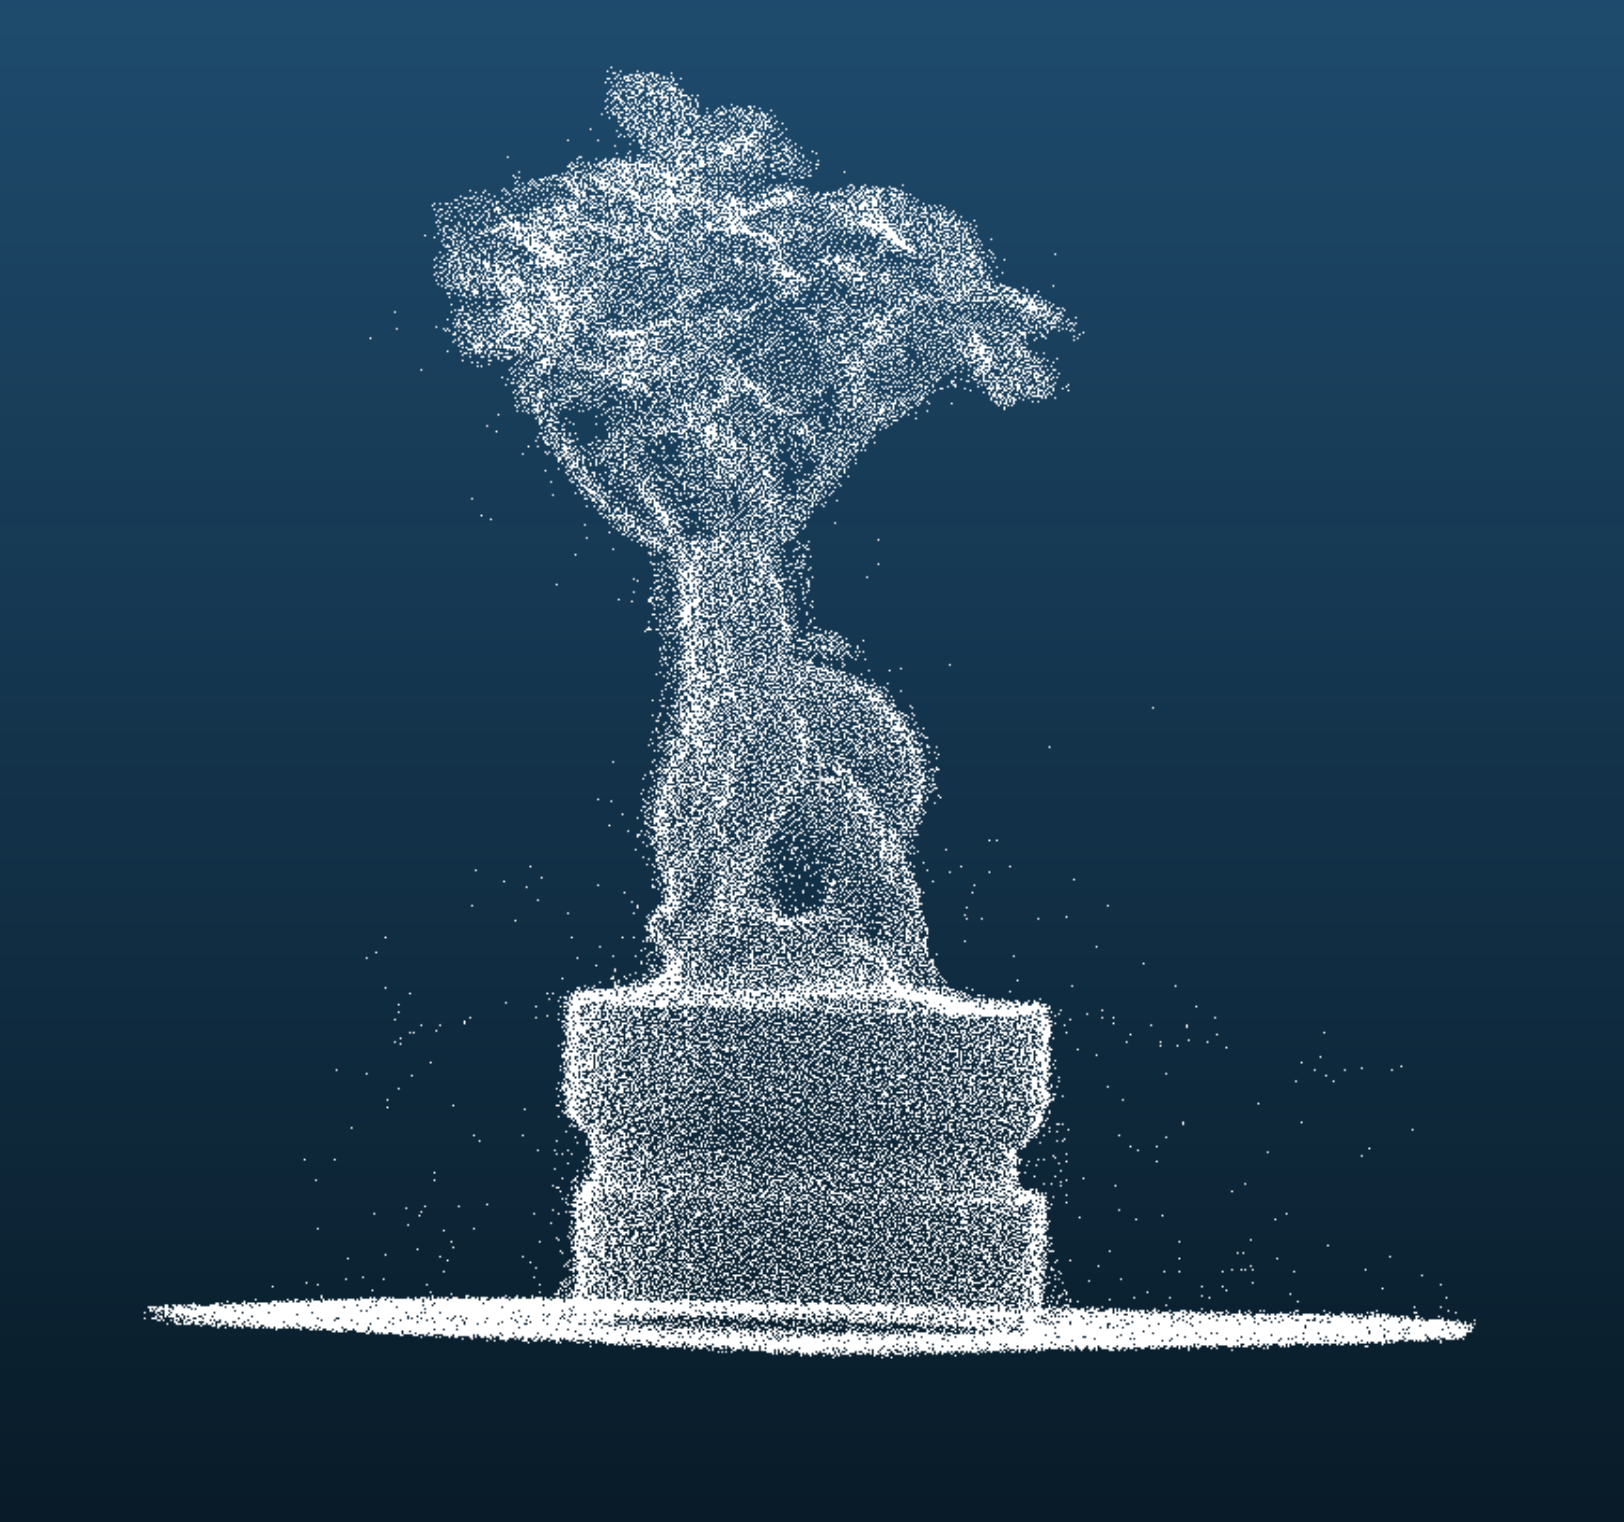
\includegraphics[width=0.9\linewidth]{complex-tree-sample.png}
\end{minipage}
\begin{minipage}{.5\textwidth}
  \centering
  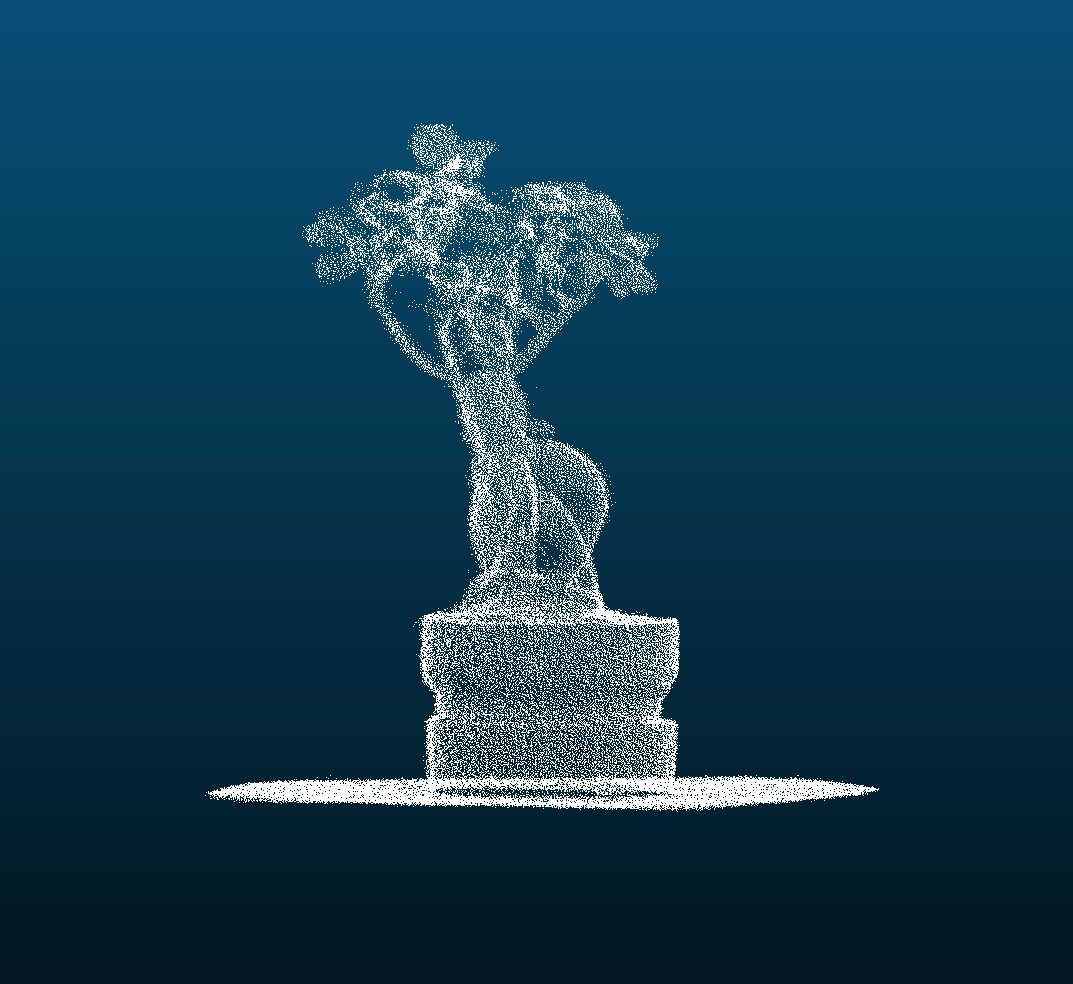
\includegraphics[width=0.9\linewidth]{after-filter.PNG}
\end{minipage}
\caption{Comparison between the point cloud before and after removing the outliers}
\label{fig:fiiter-comparison}
\end{figure}
\newpage
\subsection{Computing normals of the point clouds}
Surface normals are significant for a surface, it is important for generating good visual effects. Hence, normal estimation is a necessary preprocessing step for our project.There are many approaches for estimating the normals of the point cloud. In 1992, Hugues published his work about surface reconstruction from unorganized points \cite{14}, in this article, he estimates normals approximating a tangent plane with a regression that is computed efficiently by principal component analysis (PCA). And Alexandre presents a new method based on a robust version of the Randomized Hough Transform (RHT) which consider the filled Hough
transform accumulator as an image of the discrete probability distribution of possible normals. In the following code, we used the normal estimation function provided by PCL which is based on Hugues implementation.

The problem of determining the normal to a point on the surface is approximated by the problem of estimating the normal of a plane tangent to the surface, which in turn becomes a least-square plane fitting estimation problem \cite{15}

The solution for estimating the surface normal is therefore reduced to an analysis of the eigenvectors and eigenvalues(or PCA – Principal Component Analysis) of a covariance matrix created from the nearest neighbors of the query point. More specifically, for each point $p_i$,we assemble the covariance matrix $C$ as follows:
\begin{equation}
C = \frac{1}{k} \sum_{i=1}^{k} \cdot (p_i - \bar{p}) \cdot (p_i - \bar{p})^T , C \cdot \overrightarrow{V_j} = \lambda_j \cdot \overrightarrow{V_j}, j\in \{ 0, 1, 2 \}
\end{equation}

Where $k$ is the number of point neighbors considered in the neighborhood of $\boldsymbol{p}_i, \overline{\boldsymbol{p}}$ represents the 3D centroid of the nearest neighbors, $\lambda_j$ is the j-th eigenvalue of the covariance matrix, and $\vec{{\mathsf v}_j} $the j-th eigenvector.

For our irregular shaped tree model, Fig. \ref{fig:estimate-normal} shows the result of estimating the normals.

\begin{figure}
\centering
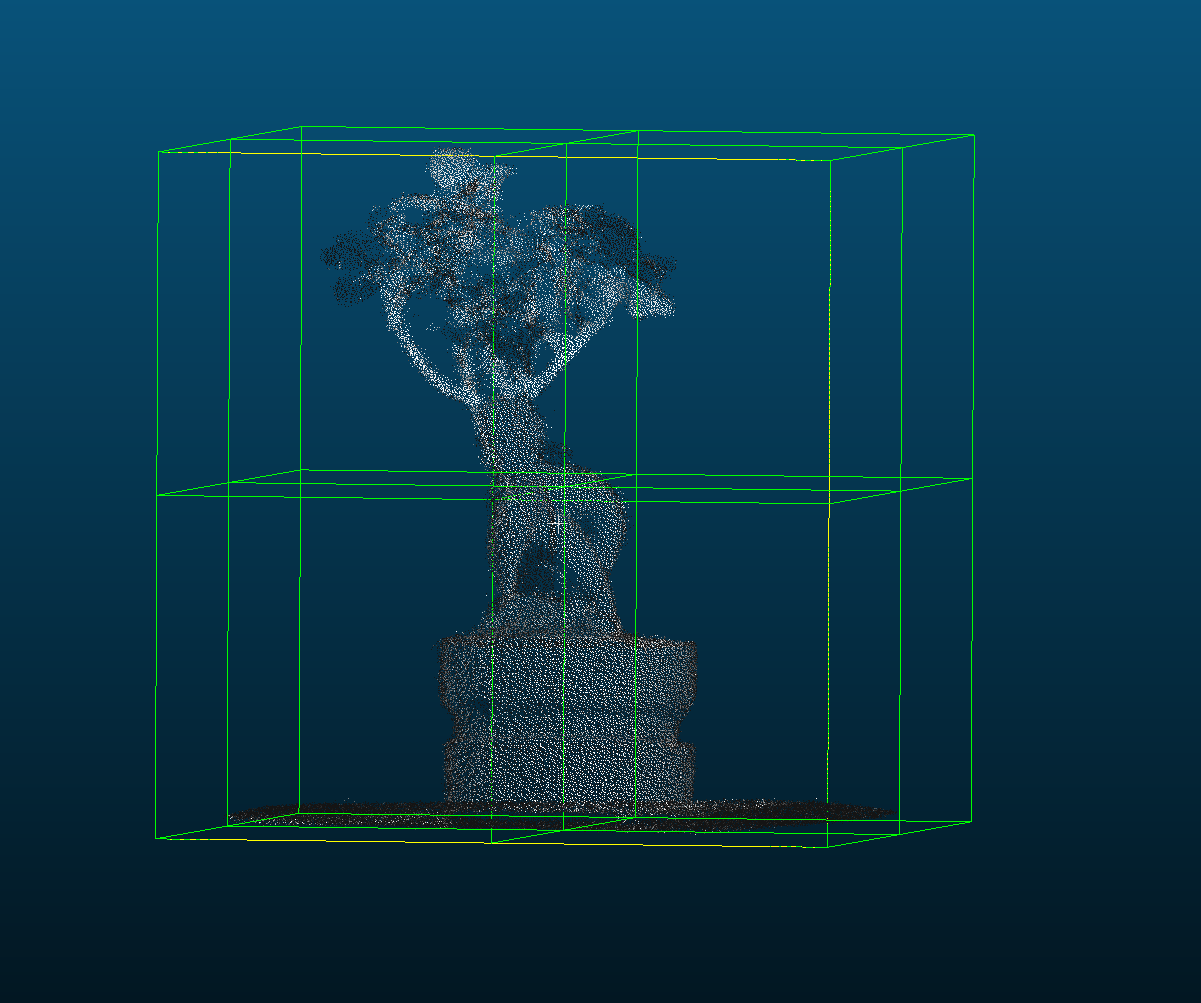
\includegraphics[scale=0.3]{estimate_normal.PNG}
\caption{Result of estimating normals}
\label{fig:estimate-normal}
\end{figure}

\subsection{Using Poisson Reconstruction to generate a mesh:}
In this step, we will implement a surface reconstruction whose input is the points with normal, and we can assume the outliers have been removed by the SOR filter. The output is a surface mesh, generated by extracting an isosurface of a surface contouring algorithm.

In 2006, Michael Kazhdan, Matthew Bolitho and Hugues Hoppe published their work of reconstructing a surface using Poisson formulation which considers all the points at once, without resorting to heuristic spatial partitioning or blending, and is therefore highly resilient to data noise\cite{16}. More specifically, his Poisson reconstruction approach includes 3 parts:

\subsubsection{Defining the gradient field.}Convolving the indicator function with a smoothing filter and consider the gradient field of the smoothed function.
\subsubsection{Approximating the gradient field. } The input set of oriented points provides precisely enough information to approximate the integral with a discrete summation. Specifically, using the point set $S$ to partition $\partial M$ into distinct patches $P_s  \subset \partial M$, we can approximate the integral over a patch $P_s$ by the value at point sample $s.P$, scaled by the area of the patch: 
\begin{figure}
\centering
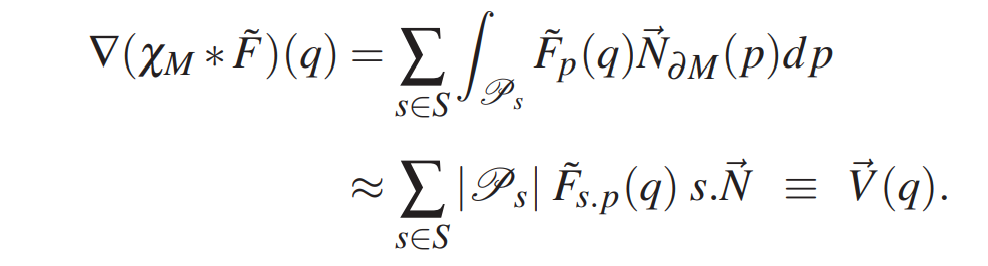
\includegraphics[scale=0.5]{equation1.PNG}
\end{figure}
 \subsubsection{Solving the Poisson problem.}
Having formed a vector field $\vec{V}$, we want to solve for the function $\tilde{X}$, such that $\nabla \tilde X $
However, $\vec{V}$ is generally not integrable (i.e. it is not curlfree), so an exact solution does not generally exist. To find
the best least-squares approximate solution, we apply the divergence operator to form the Poisson equation

\begin{equation}
\Delta \tilde X = \nabla \tilde X 
\end{equation}
\\
\\
\\
\\
\\
\\
\\
\\
The result of poisson reconstruction can be shown in Fig. \ref{fig:tree-mesh}.

\begin{figure}
\centering
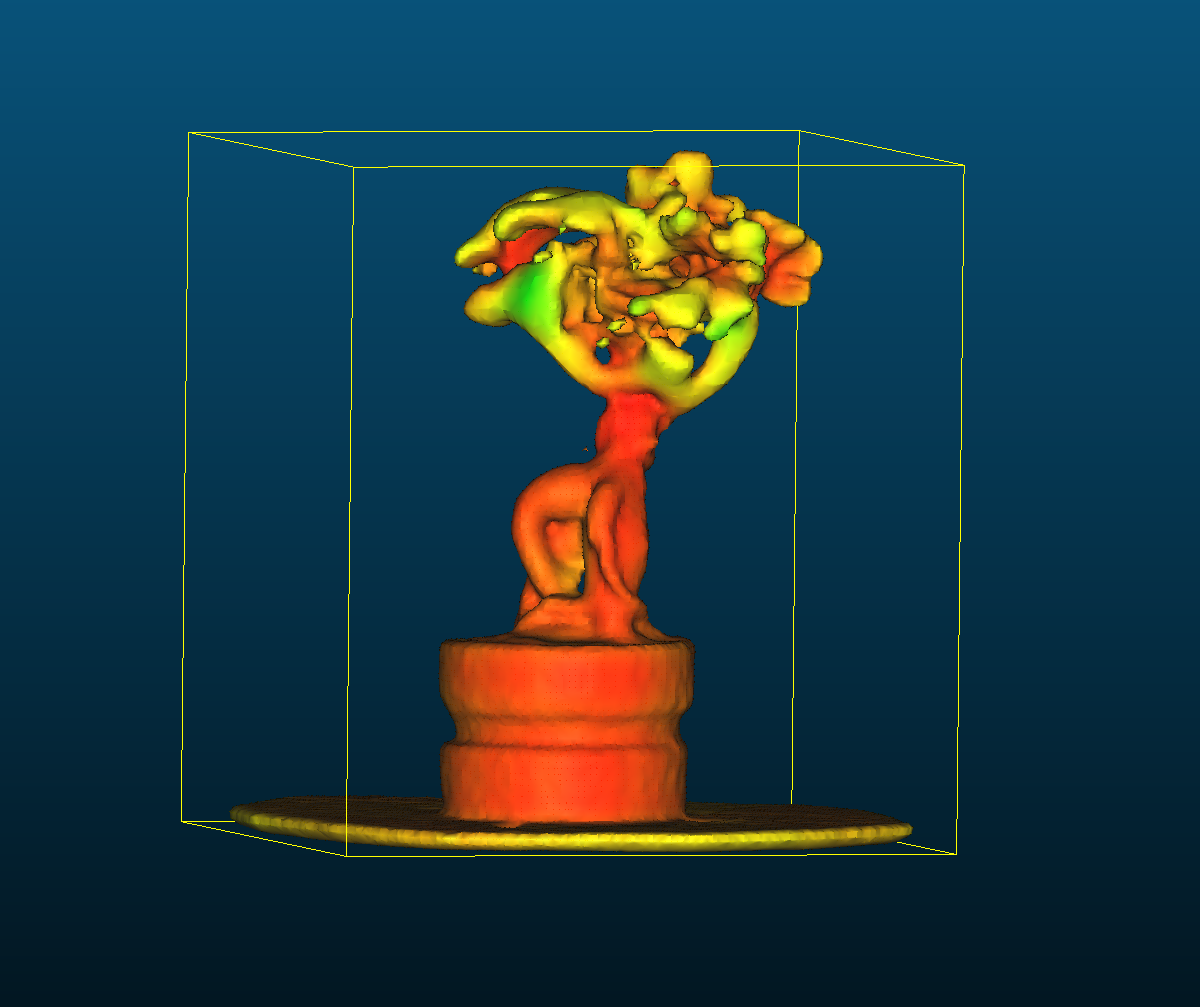
\includegraphics[scale=0.4]{tree_mesh.PNG}
\caption{Result of poisson reconstruction}
\label{fig:tree-mesh}
\end{figure}
\newpage
\subsection{Segment out the buttress part and close holes}
Using our approach, we can even calculate volume of the whole tree. If we only want to calculate the volume of the buttress part we can use the segmentation tool in CloudCompare, we segment the buttress part from the original mesh. Notice that there may be redundant part included, we can apply another segmentation on it. The comparison between before and after adjustment can be seen from Fig. \ref{fig:mesh-segmentation}. As noticed in Fig. \ref{fig:mesh-hole}, There are two significant holes on our mesh after segmentation. For our algorithm, there will be a large error if the mesh has holes. We will use Meshlab[v2016.12] to close these them. We import our mesh in the Meshlab, run the Close Holes feature under the Filter menu. 
We can adjust the thresholds of the max size for Close Holes; the holes should be closed properly, and we eventually get a watertight buttress mesh. 

\begin{figure}
\begin{minipage}{.5\textwidth}
  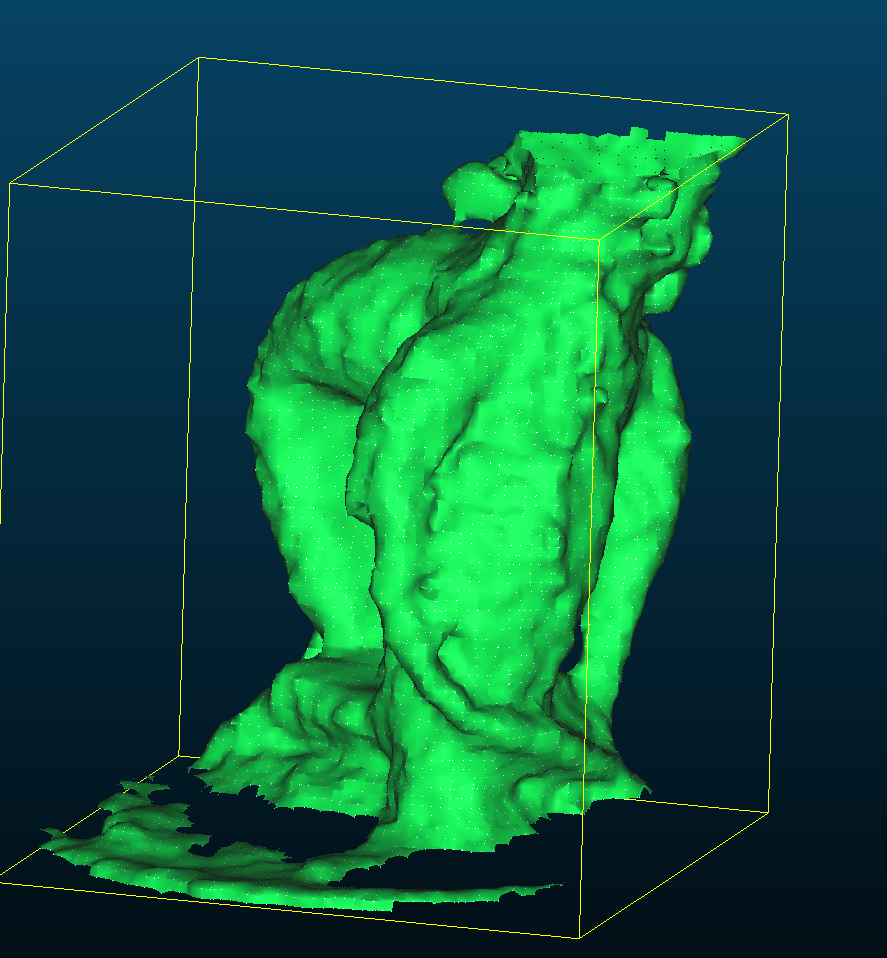
\includegraphics[width=0.9\linewidth]{segment-mesh.PNG}
\end{minipage}
\begin{minipage}{.5\textwidth}
  \centering
  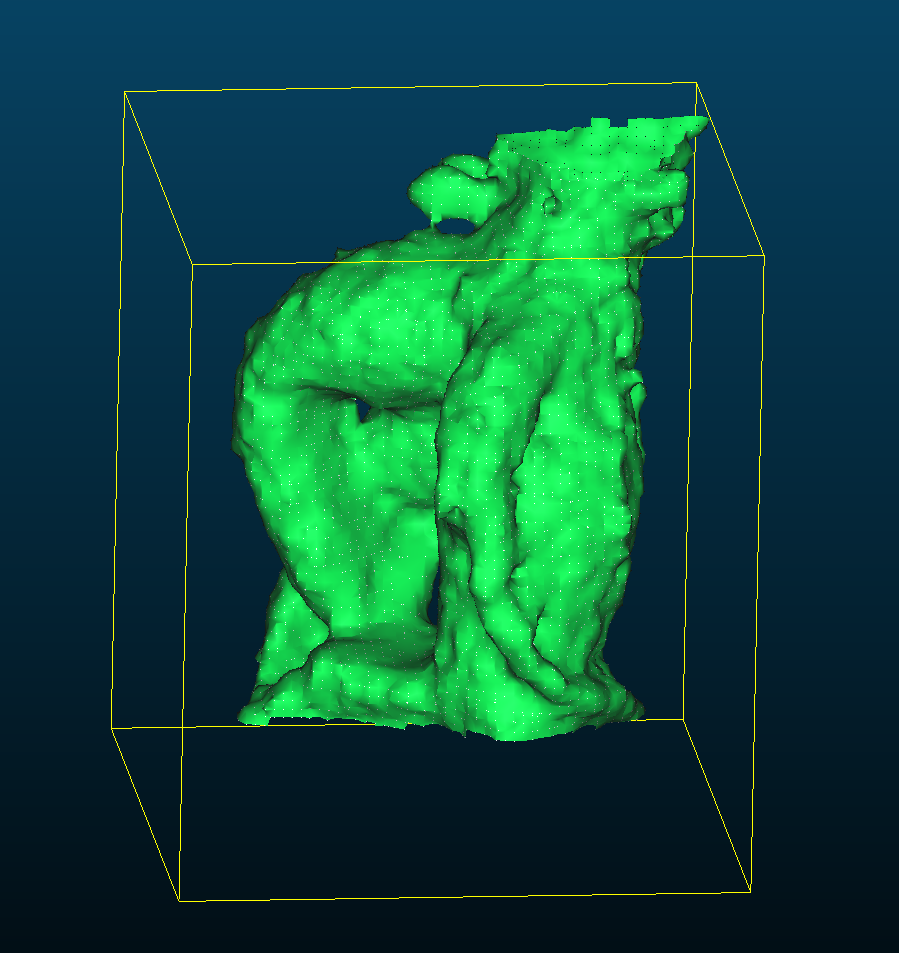
\includegraphics[width=0.9\linewidth]{adjusted.PNG}
\end{minipage}
\caption{Comparison between the mesh before and after segmentation}
\label{fig:mesh-segmentation}
\end{figure}

\begin{figure}
\begin{minipage}{.5\textwidth}
  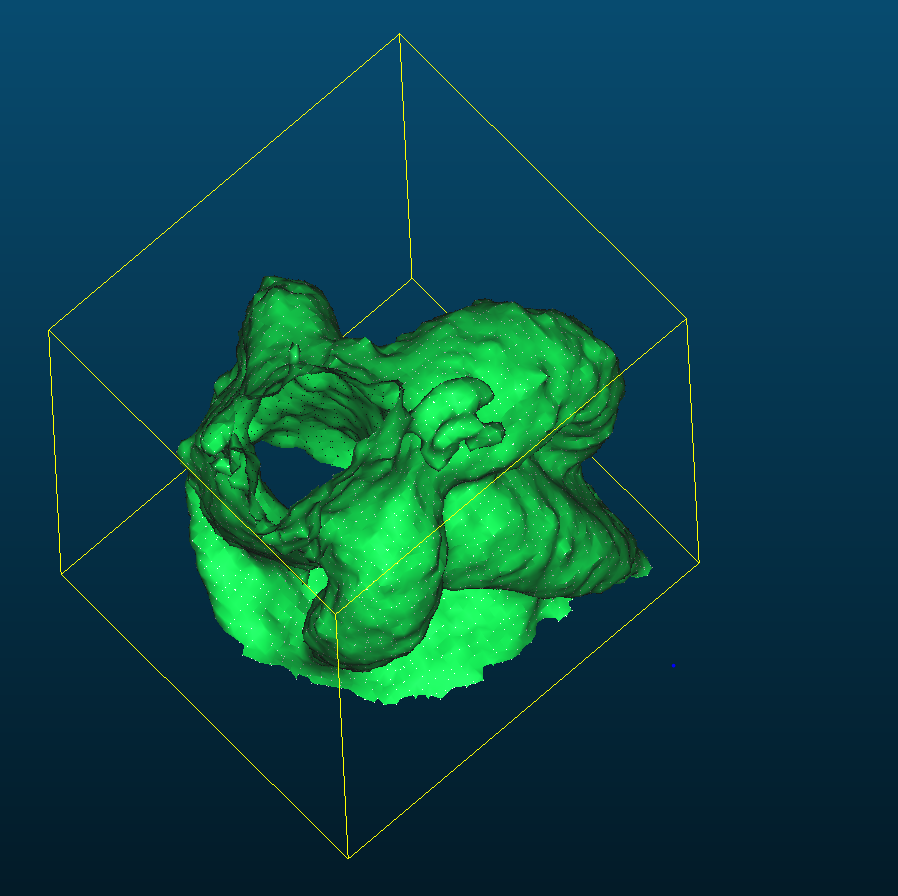
\includegraphics[width=0.9\linewidth]{meshwithhole.PNG}
\end{minipage}
\begin{minipage}{.5\textwidth}
  \centering
  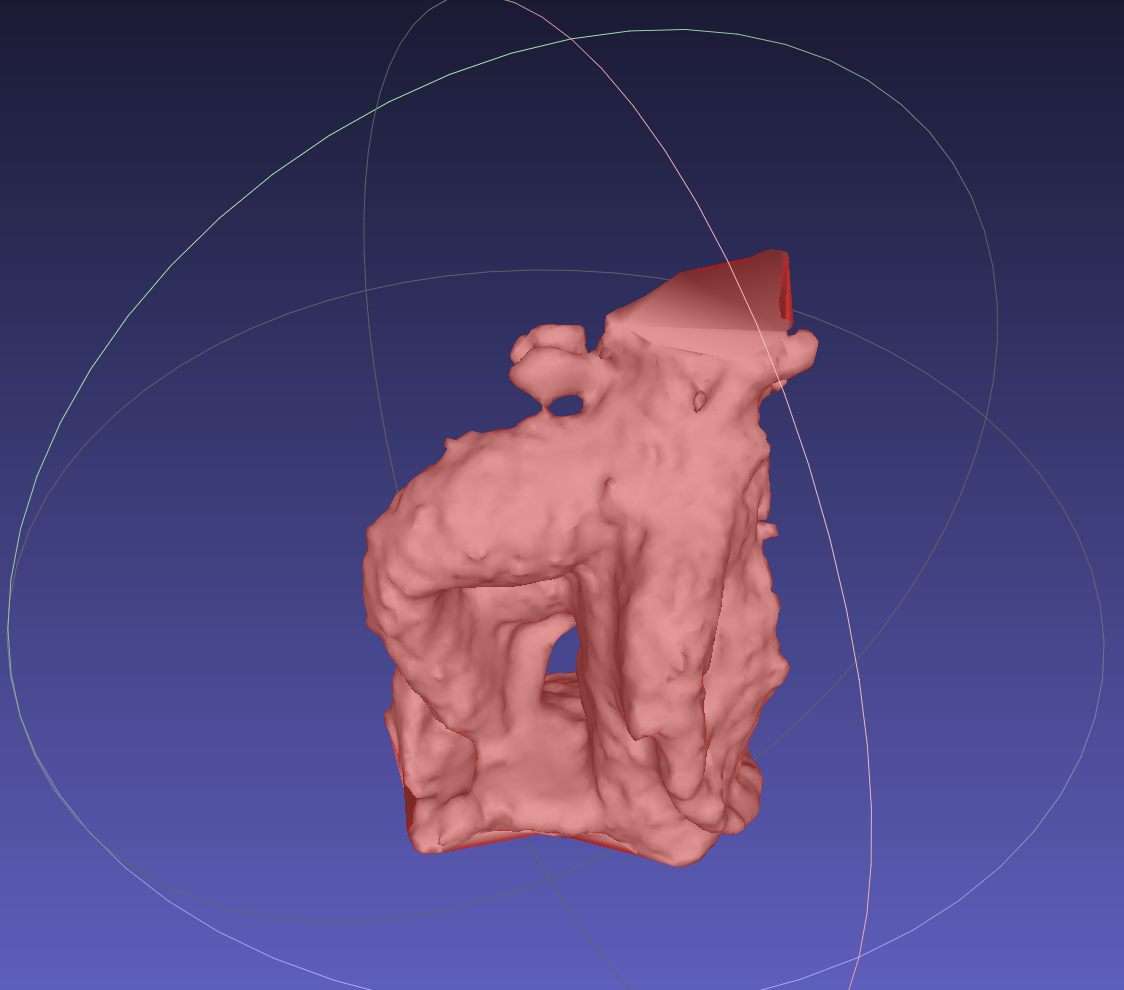
\includegraphics[width=0.9\linewidth]{Closed_hole.PNG}
\end{minipage}
\caption{Comparison between the mesh with and without hole}
\label{fig:mesh-hole}
\end{figure}

\subsection{Calculating the volume from the buttress mesh}
Since we have the accurate mesh presentation of the buttress, we use a polyhedron volume calculation algorithm introduced by Sheue-ling and James to calculate the volume\cite{17}:
The mesh surfaces consist of tons of triangles. We build up a coordinate, and connect the vertexes of triangles with the origin(0,0,0). Then we can get a tetrahedron, whose volume can be calculated by
\begin{equation}
V = \frac{1}{6}(v_1 \times v_2) \cdot v_3
\end{equation}
Using integral method, we add up all the volume of tetrahedron and the value is the volume of the whole mesh. We notice that once we build up the coordinate, each tetrahedron’s  volume has a sign so that the overlapping part will be subtract and only the inner part left. 

The final result we get from this algorithm is shown in Fig. \ref{fig:mesh-volume}.

\begin{figure}
\centering
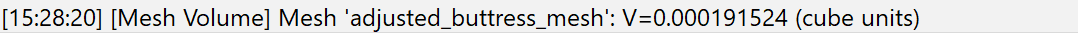
\includegraphics[scale=0.8]{finalresults.PNG}
\caption{Result of calculating the mesh volume}
\label{fig:mesh-volume}
\end{figure}

\section{Conclusion}
We presented a point cloud analysis method which can calculate the volume of any irregular-shaped buttress roots. This advantage of this method over other volume estimation methods is that this method has high accuracy all different shaped buttress. Since this method is based on Poisson Reconstruction, we can keep a high accuracy when applying this method to an irregular shaped buttress just like we shown in the article. There is still a limitation that we need to segment the buttress roots and close holes manually. In future work, we can focus on developing an automotive workflow of the buttress segmentation and hole closing.
\newpage
\begin{thebibliography}{4}
\bibitem{1}Norbert Haala, Ralf Reulke, Michael Thies, Tobias Aschoff (2004). Combination of terrestrial Laser Scanning with high resolution panoramic Images for Investigations in Forest Applications and tree species recognition.
\bibitem{2}Othmani, A., Voon, L. F., Stolz, C., Piboule, A. (2013). Single tree species classification from Terrestrial Laser Scanning data for forest inventory. Pattern Recognition Letters, 34(16), 2144-2150. doi:10.1016/j.patrec.2013.08.004.
\bibitem{3}Puttonen, E., Suomalainen, J., Hakala, T., Räikkönen, E., Kaartinen, H., Kaasalainen, S., Litkey, P. (2010). Tree species classification from fused active hyperspectral reflectance and LIDAR measurements. Forest Ecology and Management, 260(10), 1843-1852. doi:10.1016/j.foreco.2010.08.031.
\bibitem{4}Vauhkonen, J., Hakala, T., Suomalainen, J., Kaasalainen, S., Nevalainen, O., Vastaranta, M., . . . Hyyppa, J. (2013). Classification of Spruce and Pine Trees Using Active Hyperspectral LiDAR. IEEE Geoscience and Remote Sensing Letters, 10(5), 1138-1141. doi:10.1109/lgrs.2012.2232278.
\bibitem{5}Åkerblom, M., Raumonen, P., Mäkipää, R., Kaasalainen, M. (2017). Automatic tree species recognition with quantitative structure models. Remote Sensing of Environment, 191, 1-12. doi:10.1016/j.rse.2016.12.002.
\bibitem{6}G. Vosselman, B.G.H. Gorte, G. Sithole and T. Rabbani(2004), Recognising Structure in Laser Scanner Point Clouds, retrieved from https://www.researchgate.net/profile/Ben\_Gorte/publication/228875768\_Recognising\_structure\_in\_laser\_scanner\_point\_clouds/links/0c96052418a855e419000000.pdfe
\bibitem{7}Donald R. Chand, Sham S. Kapur (1970) An Algorithm for Convex Polytopes. Journal of the ACM (JACM) Volume 17 Issue 1, Pages 78-86. doi>10.1145/321556.321564
\bibitem{8}Timothy M. Chan. "Optimal output-sensitive convex hull algorithms in two and three dimensions". Discrete and Computational Geometry, Vol. 16, pp.361–368. 1996.
\bibitem{9}Euclidean Cluster Extraction Documentation. Retrieved from http://pointclouds.org/documentation/tutorials/cluster\_extraction/.
\bibitem{10}Tran, T., Cao, V., Laurendeau, D. (2015). Extraction of cylinders and estimation of their parameters from point clouds. Computers \& Graphics, 46, 345-357. doi:10.1016/j.cag.2014.09.027.
\bibitem{11}PCD Documentation. Retrieved from http://pointclouds.org/documentation/tutorials/pcd\_file\_format.php/.
\bibitem{12} Removing outliers using a StatisticalOutlierRemoval filter. Retrieved from http://www.pointclouds.org/documentation/tutorials/statistical\_outlier.php
\bibitem{13}Filter Documentation. Retrieved from http://pointclouds.org/documentation/tutorials/statistical\_outlier.php/.
\bibitem{14}Hoppe, H. (1995). Surface reconstruction from unorganized points. Ann Arbor, Mi: University Microfilms International.
\bibitem{15}Estimating Surface Normals in a PointCloud, Retrieved from http://pointclouds.org/documentation/tutorials/normal\_estimation.php
\bibitem{16}Michael K. Matthew B. Hugues H. (2006) .Poisson Surface Reconstruction. Retrieved from http://www.cs.jhu.edu/~misha/MyPapers/SGP06.pdf
\bibitem{17} Sheue-ling Lien, James T. Kajiya (1984). A symbolic method for calculating the integral properties of arbitrary nonconvex polyhedra. IEEE Computer Graphics and Applications. Volume 4, Issue 10, pages 35-42, doi 10.1109/MCG.1984.6429334
\end{thebibliography}


% \section*{Appendix: Springer-Author Discount}

% LNCS authors are entitled to a 33.3\% discount off all Springer
% publications. Before placing an order, the author should send an email,
% giving full details of his or her Springer publication,
% to \url{orders-HD-individuals@springer.com} to obtain a so-called token. This token is a
% number, which must be entered when placing an order via the Internet, in
% order to obtain the discount.

\end{document}
